This sections describes the set of demos that have been compile to exercise the OpenQuake engine. These demos can be found in a public repository in GitHub at the following link \href{http://github.com/gem/oq-engine/tree/master/demos}{http://github.com/gem/oq-engine/tree/master/demos}. Furthermore, a folder containing all of these demonstrative examples is provided when an OATS (OpenQuake Alpha Testing Service) account is requested, and it is also part of the OpenQuake engine virtual image package. These examples are purely demonstrative and do not intend to represent accurately the seismicity, vulnerability or exposure characteristics of the region of interest, but simply to provide example input files that can be used as a benchmark for users planning to employ OpenQuake in Seismic Risk and Loss Estimation studies.  

The five demos use Nepal as the region of interest. An example exposure model has been developed for this region, comprising 9144 assets distributed amongst 2221 locations (due to the existence of more than an asset at the same location). A map with the distribution of the number of buildings throughout Nepal is presented in Figure \ref{fig:expNepal}. 

\begin{figure}[ht]
\centering
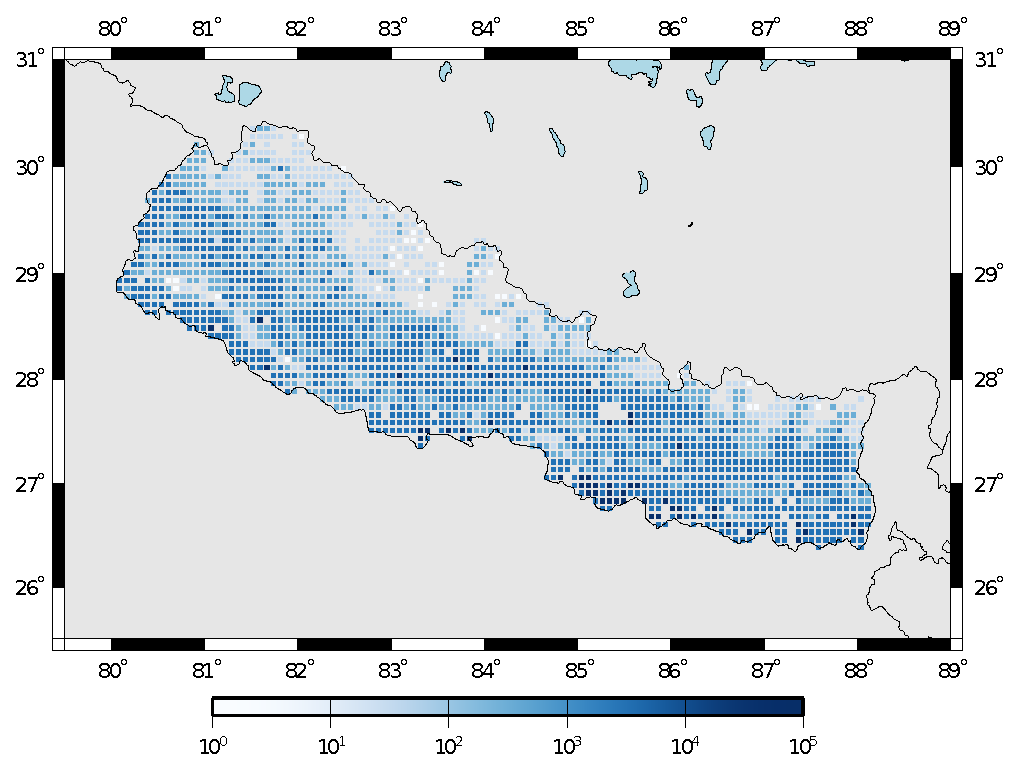
\includegraphics[width=12cm,height=8cm]{./figures/risk/NepalExposure.eps}
\caption{Distribution of number of buildings in Nepal.}
\label{fig:expNepal}
\end{figure}

The building portfolio was organised into four classes for the rural areas (adobe, dressed stone, unreinforced fired brick, wooden frames), and five classes for the urban areas (the aforementioned typologies, in addition to reinforced concrete buildings). For each one of this building typologies, a vulnerability and fragility functions was collected from the literature. These input models are only for demonstrative purposes and for further information about the building characteristics of Nepal, users are advices to contact the National Society for Earthquake Technology of Nepal (NSET - \href{http://www.nset.org.np/}{http:www.nset.org.np/}).

This section includes instruction not just to run the risk calculations, but also how to produce the necessary hazard input. Thus, each demo comprises the configuration file, exposure model and fragility/vulnerability models fundamental for the risk calculations, but also a configuration file and associated input models to produce the hazard input.

\section{Scenario Risk demo}

\section{Scenario Damage demo}

\section{Classical PSHA-based Risk demo}

\section{Probabilistic Event-based demo}

\section{Benefit/cost ratio demo}
